\documentclass[useAMS,usenatbib]{mn2e}
\usepackage{aas_macros}
\usepackage[dvips]{graphicx}
\usepackage{amssymb,amsmath}
\usepackage{times}
\bibliographystyle{mn2e}
%\documentclass[a4paper,10pt]{article}
%
\begin{document}
%
\title[Dark Matter Distribution in Dwarf Spheroidals]
      {Dark Matter Distribution in Dwarf Spheroidals}
\author[P. Steger et al.]{Pascal S. P. Steger$^{1}$\thanks{E-mail: psteger@phys.ethz.ch},
  Aaron Boley$^{2}$,
  Justin I. Read$^{1}$\\
  $^{1}$Department of Physics, ETH Z\"urich, CH-8093 Z\"urich,
  Switzerland\\
  $^{2}$Department of Astronomy; University of Florida, 211 Bryant
  Space Science Center, Gainesville, FL 32611, USA
}
%
%
\date{\today}
\pagerange{\pageref{firstpage}--\pageref{lastpage}} \pubyear{2010}
\maketitle
\label{firstpage}
\begin{abstract}
TODO: check

The dark matter distribution in dwarf galaxies expected from
simulations can then be compared with observations, allowing to check
the underlying cosmological model. When the typical distribution is
known, direct detection dark matter searches can be focused on the
densest areas, allowing for a higher annihilation detection rate.

\end{abstract}
%
\begin{keywords}
  cosmology: theory, large-scale structure of Universe --
  galaxies: dwarf spheroidals, evolution --
  methods: numerical
\end{keywords}
%
\section{Introduction}
\label{sec:intro}
TODO: overview

What is Dark Matter? Where is it? How does it influence the buildup of
structures like the Milky Way? These are simple questions that seem to
need a sophisticated way to find an answer.

\subsection{General Background}
\subsubsection{Dynamics}
TODO: intro lecture notes, get basic quantities \cite{Read2011}

TODO: 

An introduction to dynamics of bound systems is given in
e.g. \cite{TODO:BinneyTremaine}, with emphasis on galaxies.

\subsubsection{Cosmological Models}
TODO: intro Weinberg \cite{TODO:Weinberg}

Principles of physical cosmology are handled in e.g. \citep{TODO:Peacock}
The constraints from 5 year WMAP can be found in \citep{Komatsu2009}

\subsubsection{Structure Formation}
A review of how we think structure formed through the history of the
universe is found in \cite{TODO:padmanabhan}

\subsection{Dark Matter}
TODO: overview (Jungmann1996)


The current measurements \citep{Komatsu2009} indicate that 83\% of the
matter density is not interacting with baryonic matter except through
gravity and not emitting light, therefore called dark matter.

\subsubsection{Evidence for Dark Matter}
TODO: formulation

TODO: \citep{Jungman1996} Several objects in gravitationally bound
systems were found to move faster than the escape velocity determined
by the potential of the luminous parts. The velocities of galaxies in
clusters e.g. led to the notion of {\sc dark matter}
\citep{Zwicky1933}. Furthermore, galactic rotation curves should show
$v(r)\propto\sqrt{M(r)/r}$, with $v(r)\propto r^{-1/2}$ outside the
visible part; instead in most galaxies it rises to a maximum value and
stays approximately constant out to the edges of the galaxy. This
implies $M(r)\propto r$ or $\rho(r)\propto r^{-2}$.

The bullet cluster \cite{Clove2006} indicates that dark matter is some
new particle rather than an effect from modified gravity.

\subsubsection{Models}
TODO: overview
TODO: references
* MACHOs
* WIMPs
* HDM, WDM, CDM, LCDM

Hot dark matter (HDM) consists of a particle type that is still freely
streaming, as are the neutrinos.  Cold dark matter has decoupled from
the temperature field in the early universe and started to form small
structures, which merge into bigger ones.  Warm dark matter is in
between these two extremes.

\subsubsection{Possibilities for Detection}
TODO: references

Experiments to detect dark matter directly are described e.g. in \citep{Schnee2011}. One generally differs between direct and indirect detection:
* direct:
  - annihilation signal from high-energetic particles generated during smash
  - interaction with detector material needed
  - sensitive detectors, needs shielding from cosmic rays and radioactive materials

* indirect
  - dynamics
  - lensing
  - 

  To actually detect dark matter, one is interested in the expected
  density distribution of dark matter in galaxies, as
  \citep{Navarro1996} shows.
\subsection{Dwarf Galaxies}
TODO: (TODO: check reference) \citep{Ostriker2003}. Let us adhere to
the definition of dwarf galaxies as the smallest galaxies in the
Universe, with dynamical masses $10^6M_\odot-10^8M_\odot$ determined
from visible components, while star masses range from
$\sim1000M_\odot$ to $10^7M_\odot$, and almost no gas is visible.

TODO: overview is given in \citep{Mateo1998}. Star formation histories
of the dwarfs is covered e.g. in \citep{Skillman2005} and
\citep{Dolphin2005}, kinematics in \citep{Walker2009} and
\citep{Simon2007}, and their orbits in \citep{Lux2010}.

Elliptical galaxies with luminosities below $10^9L_\odot$ can be split
in two families, one of which has much lower surface brightness and
bigger radii than the other. This family is named dwarf
spheroidals. They are so faint in fact that they are only detected in
the neighborhood of the Milky Way, with an estimated number count of
50-100 \citep{Belokurov2007}. They differ from other gravitationally
bound systems in that they consist mostly of dark matter; more
luminous halos show comparable densities of baryonic and dark matter
in the inner regions.

\subsubsection{Defining Properties}
A dwarf galaxy can be defined in several manners. Normally any galaxy
with mass $<10^{11}M_\odot$ is called \"dwarf\". But as there can be
distinguished two families of galaxies below that mass, one has to
constrain further. In this work the notation dwarf is used for the
smallest galaxies known in the Universe, with masses detected through
the dynamics of the visible part in the interval from $10^6M_\odot$ to
$10^8M_\odot$, a small amount of observable gas, and stellar masses
from $1000M_\odot$ to $10^7M_\odot$.
%
\subsubsection{Observations}
Galaxies with a mass as low as stated before, the luminosity is
expected to be very low as well. This induces that only nearby dwarf
galaxies can be observed with current observational instruments.

Observations show only of order $100$ dwarfs in the Milky Way halo,
although there should be thousands of them. This discrepancy is
generally known as the ``missing satellites problem'',
\citep{Moore1999}, \citep{Klypin1999}. Recently, wide area surveys
discovered more and more dwarfs, \citep{Belokurov2007},
\citep{Belokurov2009}, \citep{Belokurov2010}.

Cusp-Core problem: Observations show a core in the central parts of
rotationally supported dwarf galaxies, which is in contrast to theory
predicting cuspy profiles for dark matter only profiles,
\citep{Moore1994}, \citep{Flores1994}, \citep{Moore1999a}.

Looking at simulated galaxies that are not necessarily rotationally
supported, additional constraints as to which properties distinguish
cores and cusps can be found. Baryons do play an non-neglectible role
in dwarf dynamics, generating cores from cusps via either
non-adiabatic contraction or recurring baryonic in-/outflow
\citep{Read2005}, which could render the cusp-core problem
pointless. This is in fact seen in simulations \citep{Mashchenko2008},
\citep{Governato2009}, which shows that the early assumption that
baryon physics has only small influence were wrong
\citep{Navarro1996}, \citep{Gnedin2002}.

\subsection{Globular Clusters}
Massive star clusters in the halo of the Milky Way - of which some 150
are detected by now \cite{TODO} - show a mass in stars that is
comparable to the dwarf spheroidals, typically $10^5$ to
$10^6M_\odot$. The resemblance is going further as they have a similar
age; they are mostly old, as old as the Universe itself
\cite{TODO}. The big difference lies in the fact that they show little
to no evidence for dark matter in them, whereas dynamics of dwarf
spheroidals implies a mass fraction of $90\%$ in dark matter.

Observations of globular clusters in our Galaxy are given in
\citep{Zinn1985} and \citep{DeAngeli2005}.

Why should stars form in environments with such a wide spread in
density? Is there a connection between dwarf spheroidals and globular
star clusters? Given there is one, how can it be determined
qualitatively and quantitatively? It has been proposed \cite{TODO}
that one is the evolved form of the other; or \cite{TODO} that they
form in different environments.

By extracting basic properties that differ in between globular star
clusters and dwarf spheroidals, one can try to answer that
question. The temporal evolution of the defined substructures gives
hints as to whether they represent different phases in an evolutionary
path.

The density of globular clusters is such that in a typical patch of
the LCDM Universe of size $1\rm Mpc$ at $z=10$ contains a few of them
\citep{Boley2009}.

\subsection{Simulations}
The general paradigm behind simulations is as follows:

Take observations of todays structures and try to recover them. This
is done via setup of initial conditions similar to the ones that one
can see in the cosmic microwave background. There are two different
approaches, one assuming gaussianity, the other a little correction
term $f_{\rm NL}$.

These initial conditions are power spectra for the modes of
displacement in density and velocity, modeled on a grid of $N^3$
particles in a box. The box is assumed to repeat itself in each
cartesian coordinate, effectively forming a hypertorus.

The simulation is then started and begins to calculate 
\begin{itemize}
\item gravitational forces between particles
\item hydrodynamical quantities, either for hydro particles or on a mesh
\item the resulting changes for the next step
\end{itemize}

A review of how structure formation can be modeled by numerical means
is found in \citep{Bagla2005}.
\subsubsection{Ideas}
TODO: all
\subsubsection{Scopes}
TODO: all
\subsubsection{Paradigmas}
TODO: all

Collisional codes follow each of the particles directly, while
collisionless simulations follow a smaller number of particles that
are actually expected to be in the system. Collisional codes are used
to follow systems in which close encounters play a significant role
and need to be resolved, i.e. when relaxation time is of order of the
simulation timestep. In collisionless simulations one tries to model a
continuum distribution by sampling only a small number of
particles. Dark matter as a pressureless fluid is treated by this
paradigma.

$N$-body simulations do use a discrete sample of points in phase space
to follow the evolution of the whole system. The track of a particle
is determined by the gravitational force on it generated by the
gravitational potential of all other particles. Any code that
calculates this force and then follows the particle path and thereby
integrates Poisson's equation is called a Poisson solver.

TODO:
*P3M

Particle-Particle-Particle-Mesh uses direct summation of forces
between all (star/dark matter) particles.

*PM

*{\sc Sph} Smoothed particle hydrodynamics approaches the fluids by
particles representing volume elements, and calculates the
hydrodynamical forces from a discrete form of the Euler equations.

*AMR

Adaptive mesh refinement describes an advanced technology to follow
the liquid more accurately: The mesh is refined in the vicinity of
high overdensity, allowing for correct capture of accretion, shock
waves, and other small features.

\subsubsection{codes}
TODO: overview, references
*GADGET
{\sc Gadget} is a {\sc Sph} code.
Two versions:
Gadget 2
Gadget 3
- TODO: changelog
*{\sc Ramses}

{\sc Ramses} \citep{TODO} uses adaptive mesh refinement technique to
handle hydrodynamic properties. Its hydrodynamical solver involves a
second order Godunov scheme.

*ENZO, GASOLINE,...
%		

\subsection{Overview this work}


\subsubsection{TOC}
This work is organized in the following way: After this introduction
with an overview over the widespread field of dark matter research and
methods of numerics in cosmology, we start by describing the
simulations performed in section \ref{sec:data}, followed by a short
explanation on the methods in section \ref{sec:meth}. Then we focus on
results: section \ref{sec:res} first concentrates on halo finding
performance and general properties of the halos in the high
resolution, hydrodynamical run, both for dark matter/stars and
gas. This is compared with the properties found in the dark matter
only run, allowing to draw conclusions on the influence of baryons.


\subsubsection{Novelties}
TODO: all


%
%% SIMULATIONS
%
%
\section{The Data}
\label{sec:data}
\begin{figure}
  \begin{center}
    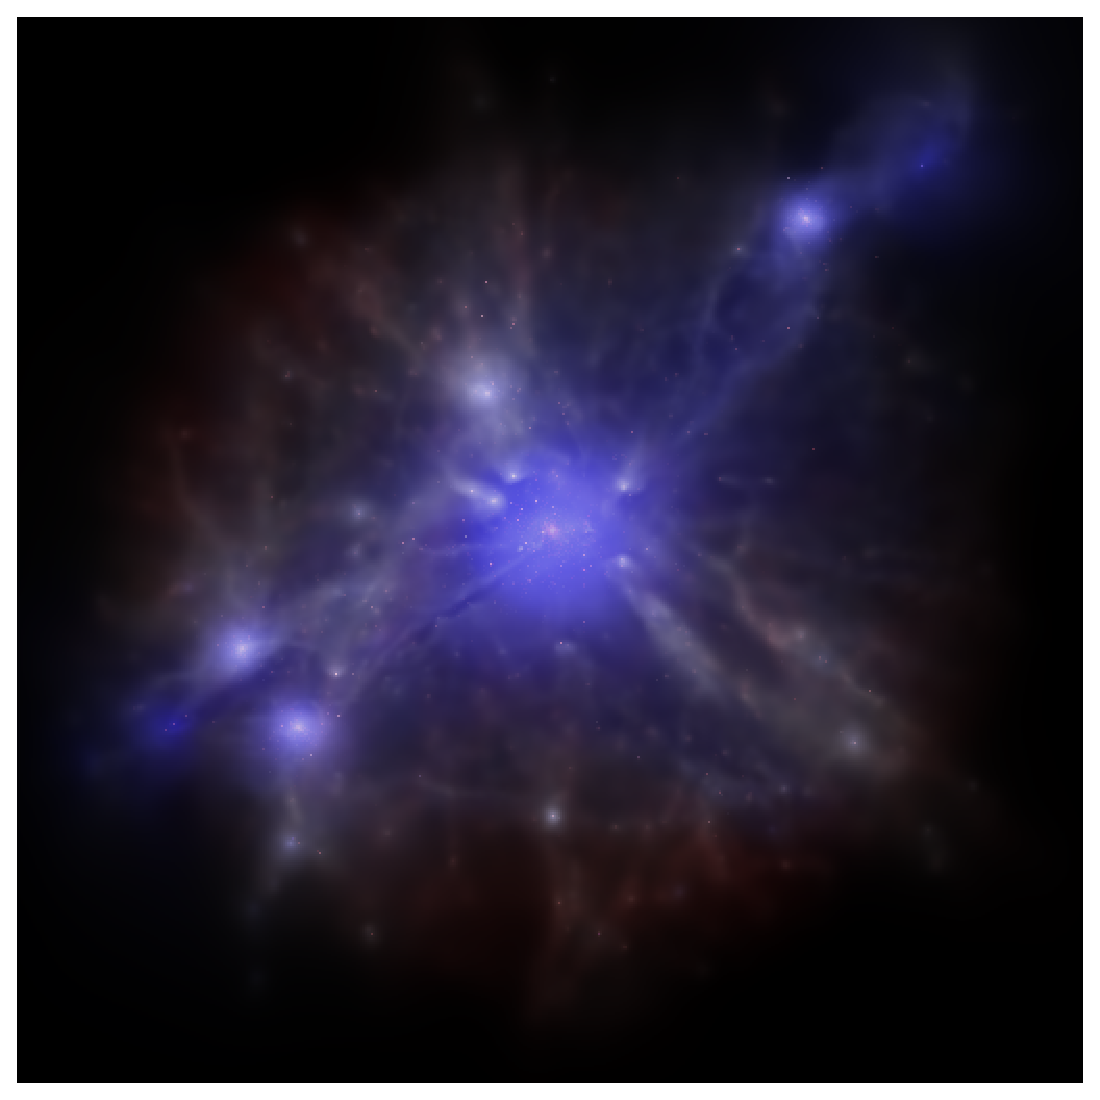
\includegraphics[width=0.45\textwidth]{fig/splotch/out.eps}
  \end{center}
  \caption{ \label{fig:splotch} Visualization by ray-tracing of one of the dwarf spheroidals in the high resolution hydro run. The visible box size spans a range of $TODO\,{\rm Mpc}/h$.}
\end{figure}
%
TODO: overview


\subsection{The Simulations}
Three simulations were run for this project. The main simulation was
run with high resolution with nonequilibrium physics. For comparative
reasons the same resolution was used for a dark matter only
simulation, and convergence was investigated by a comparing that one
to a lower dark matter only simulation. All simulations used the same
cosmology, as follows.

\subsubsection{Cosmological Parameters}
The high resolution hydrodynamical simulation was run with WMAP-5
concordance cosmology parameters, i.e. $\Omega_\Lambda=0.742$,
$\Omega_M=0.258$, $\Omega_b=0.045$, $h=$, $\sigma_8=1.0$.

\subsubsection{Initial Conditions}
Initial conditions were generated with {\sc Cosmics}
\citep{Bertschinger1995}, for a box of $1{\rm Mpc}/h$ boxlength, at
$z=1000$, with a low resolution boundary layer of $128^3$ equivalent
particles and an inner high resolution region of $256^3$
particles. The dark matter only, high resolution run was performed
with $256^3$ particles on the whole box. Convergence studies were
performed by comparing it to an even higher resolution run of $512^3$
dark matter particles, run at single precision only due to restricted
memory.

\subsubsection{Stepping, motivation for stop @ z=10}
The simulation is run from $z=1000$ down to $z=10$, with outputs on
$30$ equally spaced intervals from $z=100$ to $z=10$, each further
refined into 10 smaller snapshots, allowing to track specified
structures back in time.

It has been shown in \citep{Boley2009} that in a typical volume of
$1{\rm Mpc}/h$ at $z\sim10$ there should be a few dwarf spheroidal
galaxies present. Thus the progenitors of todays dwarfs were generated
before reionization. This influence on the baryonic component will be
considered in future work.

\subsubsection{Simulation physics}
TODO: ram pressure, SN feedback, AGN, black holes, star formation recipe

Active galactic nuclei emit energy during accretion of material, which
is fed back into the surroundings. The main effect is

\subsubsection{Nonequilibrium gas physics} {\sc Ramses} is used in a
augmented version which follows nonequilibrium physics, namely the gas
of $e$, {\sc Hi}, {\sc Hii}, {\sc HEi}, {\sc HEii}, {\sc HEiii},
H$^-$, H$_2$, and $H_2^+$.

\subsection{Higher Resolution}
TODO: all

We use significantly higher resolution than was previously performed
\citep{Boley2009}, with non-equilibrium physics included
\citep{Abel1997}.

The force resolution (Plummer's equivalent length) in the highest
resolution mesh is $4pc/h$ at $z=10$, which sets a restriction on the
determination of densities in the inner regions of the smallest
halos. It is indicated as a vertical line in the graphs of radial
profiles.

\section{Methods}
\label{sec:meth}
TODO: ov
\subsection{Definitions}
TODO: all

* spherical overdensity
* 
\subsection{Halo Finding}
TODO: all

The simulation outcome by itself shows only properties of individual
dark matter particles, and additionally a mesh for the hydrodynamical
constituents. One is interested in bound substructures, which have to
be found first. To do so, a halo finder needs to be invoked.

* FOF

The friend-of-friends algorithm as e.g. described in \citep{Press1982}
starts with a particle and searches for its nearest neighbor, out to a
predefined radius. After doing this iteratively, all particles
connected by such a chain are considered to lie within the same
halo. This procedure works well for isolated halos only; two nearby
halos connected by a filament could be detected as one structure only.

* HOP

{\sc Hop} from the {\sc Ramses} toolkit starts off by computing the
density around each particle with an adaptive kernel, then hop to the
neighbor particle at highest density, and assigning all particles
ending at the same point to the same structure. Breaking up due to
local density maxima is overcome by merging two groups if the density
of the boundary layer between them lies above a given threshold.

* watershed

The watershed algorithm \citep{TODO} starts from the density maxima as
leaves of the halo/subhalo tree. Stepping further out, all material in
the same potential pot is assigned to the respective maxima. As soon
as a neighbor maximum is encountered, both halos form an additional
leave in the tree.

* SOD

The spherical overdensity algorithm as introduced by \citep{Lacey1994}
grows a sphere around particles at density minima and stops if the
mean density falls below a threshold. This procedure is repeated with
the remaining particles until no structure with a minimum number of
particles is found anymore. It does not handle correctly the cases of
mergers, yielding a halo position in the middle of both merging halos.

Here the {\sc AHFstep} algorithm of the simulation code {\sc Amiga} is
used. It showed superior capabilities with mock halos and subhalos
\citep{TODO}. The {\sc Ramses} simulation snapshots are first
converted to Gadget format, allowing a simple read-in for {\sc
  AHFstep}.

The prospective halo centers can be defined in several ways: by the
position of the center of mass, the center of the potential or the
density maximum. Visually best agreement with dark matter density
projection was found for the position of maximal density.

An additional iterative procedure excludes all particles which are
kinematically unbound: if the kinetic and internal energy (for hydro
particles) exceed the potential energy, the particle is removed, the
potential recalculated and further unbound particles excluded.

TODO: for high mass/low mass systems

{\sc AHFstep} outputs a bunch of quantities, for the next steps only
position and virial radius (inside which $\Delta\rho=200$) are used.

Additional displacements with respect to the densest point are
corrected with an additional shrinking sphere algorithm: It starts
from the center of mass of all particles in a sphere of radius $r_{\rm
  vir}$, then rescales the radius to $r_{i+1}=(1-f)r_i$, and considers
only particles inside the smaller sphere to find the center of mass in
the next step, until the positions converge to $(\Delta x_{i\to
  i+1}-\Delta x_{i-1\to i})/\Delta x_{i\to i-1}<\varepsilon$. The two
parameters $f$ and $\rho$ are not restricted by a physical argument
and thus have been chosen such that for the majority of massive halos
convergence was reached in $<100$ steps, with displacements
$<0.1r_{\rm vir}$.

\subsection{Halo Selection}
We are interested in the inner density profile of dwarf spheroidals,
therefore, only halos with virial mass above $10^7M_\odot/h$ and no
host halo are considered further. Their main properties are listed in
table \ref{tab:haloprop}.

TODO: update table
\begin{table}
  \begin{center} \begin{tabular}{lccccccccr} \hline Simulation &
      ID & $M_{\rm vir} / h^{-1}{\rm M}_\odot $ & $R_{\rm vir} /
      h^{-1}{\rm Mpc}$ &x&y&z& $f_{DM}$ & $f_{gas}$ & $f_{stars}$ \\ 
      \hline
      hydro & 1 & $TODO$ & $TODO$ & x & y & z & TODO & TODO & TODO\\

      \hline
    \end{tabular} \end{center}
  \caption{\label{tab:haloprop}Properties of the selected halos. $M_{\rm vir}$ and $R_{\rm vir}$ are the virial mass and radius of the halos.}
\end{table}


\section{Results}
\label{sec:res}
TODO: ov

\subsection{Halo finding}
\begin{figure}
  \begin{center}
    
\includegraphics[width=0.45\textwidth]{fig/a.eps}%fig/vis_proj_dm_sod_ahf.png}
  \end{center}
  \caption{\label{fig:vis_proj_dm_sod_ahf}Positions of the halos detected by SOD (blue circle) and {\sc Ahf} (red crosses) on top of dark matter density}
\end{figure}


\begin{figure}
  \begin{center}
    
\includegraphics[width=0.45\textwidth]{fig/a.eps}%vis_proj_gas_sod_ahf.png}
  \end{center}
  \caption{\label{fig:vis_proj_gas_sod_ahf}Positions of the halos detected by SOD (blue circles) and {\sc Ahf} (red crosses) on top of gas density}
\end{figure}

\begin{figure}
  \begin{center}
    
\includegraphics[width=0.45\textwidth]{fig/a.eps}%hist_shrsph.png}
  \end{center}
  \caption{\label{fig:hist_shrsph}Distribution of additional position correction by shrinking sphere algorithm.}
\end{figure}



\subsection{DM density profile}

TODO: all

method:

\begin{figure}
  \begin{center}
    
\includegraphics[width=0.45\textwidth]{fig/a.eps}%dm_prof.png}
  \end{center}
  \caption{\label{fig:dm_prof}Dark matter density profile of the five most massive halos}
\end{figure}

\begin{figure}
  \begin{center}
    
\includegraphics[width=0.45\textwidth]{fig/a.eps}%r_core_m.png}
  \end{center}
  \caption{\label{fig:r_core_m}Core radius versus mass for all halos.}
\end{figure}

\begin{figure}
  \begin{center}
    
\includegraphics[width=0.45\textwidth]{fig/a.eps}%hist_slopes.png}
  \end{center}
  \caption{\label{fig:hist_slopes}Distribution of slopes for core and outskirt}
\end{figure}

\begin{figure}
  \begin{center}
    
\includegraphics[width=0.45\textwidth]{fig/a.eps}%star_prof.png}
  \end{center}
  \caption{\label{fig:star_prof}Density profile of star particles in the five most massive halos}
\end{figure}

\begin{figure}
  \begin{center}
    
\includegraphics[width=0.45\textwidth]{fig/a.eps}%hist_mstarbymdm.png}
  \end{center}
  \caption{\label{fig:hist_mstarbymdm}Fraction of stellar mass to dark matter mass in all halos with $M<TODO$}
\end{figure}


\subsection{Gas Density Profile}
TODO: all

\begin{figure}
  \begin{center}
    
\includegraphics[width=0.45\textwidth]{fig/a.eps}%gas_prof.png}
  \end{center}
  \caption{\label{fig:gas_prof}Density profile of gas in the five most massive halos}
\end{figure}

\begin{figure}
  \begin{center}
    
\includegraphics[width=0.45\textwidth]{fig/a.eps}%metal_2.png}
  \end{center}
  \caption{\label{fig:metal_2}Radial dependence of star metallicities for $metal>metal_*$ and $metal<metal_*$}
\end{figure}


\subsection{Temporal Evolution}
TODO: all
The simulation produced output snapshots in regular intervals, allowing for an investigation on how the different values change with epoch.

\begin{figure}
  \begin{center}
    
\includegraphics[width=0.45\textwidth]{fig/a.eps}%corerad_temp.png}
  \end{center}
  \caption{\label{fig:corerad_temp}Core radius as a function of time, for the five most massive halos}
\end{figure}


%
\section{Summary and Discussion}
\label{sec:sum}
%
TODO: overview
\subsection{Impacts on Formation History}
TODO: all

\subsection{Further Evolution down to z=0}
TODO: all

\subsection{Local DM Density}
TODO: all
%
%
\section*{Acknowledgements}
\label{sec:ack}
%
TODO: Read, Boley, Garbari, Hobbs, Teyssier

S. Garbari provided a prototype algorithm for the correction of the
prospective halo centers.  A. Boley gave numerous hints of technical
nature, and provided sample scripts for starting analysis.
%
\section{Appendix: Numerical Robustness, Convergence}
\label{sec:app}

The low resolution simulation was used to check convergence of the high resolution dark matter only simulation.

\begin{figure}
  \begin{center}
    
\includegraphics[width=0.45\textwidth]{fig/a.eps}%corr_r_core.png}
  \end{center}
  \caption{\label{fig:corr_r_core}Correlation between core radii detected in low resolution (abscissa) and high resolution run (oordinate).}
\end{figure}


%
%%% end of content
%
% sample figure inclusion statements
%
% \begin{figure}
%   \begin{center}
%     \includegraphics[width=0.45\textwidth]{fig/label}
%   \end{center}
%   \caption{\label{fig:label}small figure, width one column}
% \end{figure}
%
% spanning two columns
%
% \begin[ht]{figure*}
%   \begin{center}
%     \hspace{1cm}
%     \includegraphics[width=0.85\textwidth]{fig/label}
%   \end{center}
%   \caption{\label{fig:label}big figure, width one page}
% \end{figure*}
%
%
\bibliography{main}
all references from reading list +both Oh2010


%
\label{lastpage}
\end{document}
